\section{MSLPlot\-Window  Class Reference}
\label{classMSLPlotWindow}\index{MSLPlotWindow@{MSLPlot\-Window}}
{\tt \#include $<$guiplanner.h$>$}

Inheritance diagram for MSLPlot\-Window::\begin{figure}[H]
\begin{center}
\leavevmode
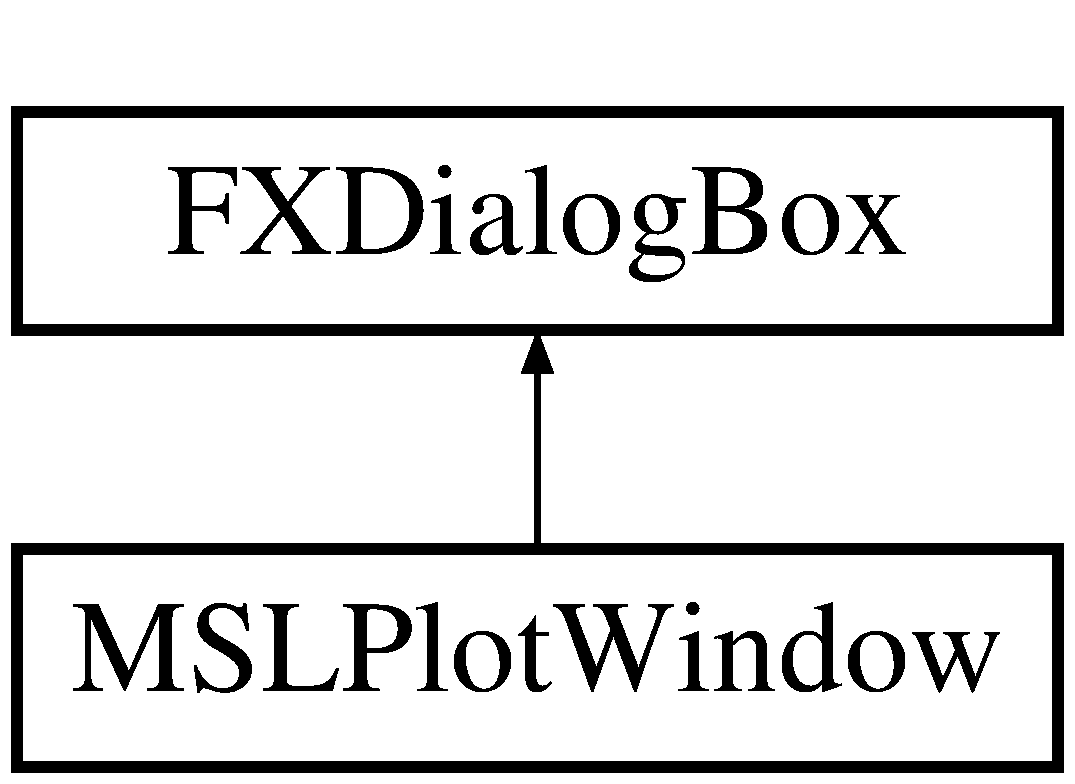
\includegraphics[height=2cm]{classMSLPlotWindow}
\end{center}
\end{figure}
\subsection*{Public Methods}
\begin{CompactItemize}
\item 
long {\bf on\-Paint} (FXObject $\ast$,FXSelector, void $\ast$)
\item 
long {\bf on\-Cmd\-Print} (FXObject $\ast$,FXSelector, void $\ast$)
\item 
{\bf MSLPlot\-Window} ({\bf MSLPlanner\-Window} $\ast$owner)
\item 
void {\bf draw\-Page} (FXDC \&dc, FXint w, FXint h, FXint tx=0, FXint ty=0)
\end{CompactItemize}


\subsection{Constructor \& Destructor Documentation}
\index{MSLPlotWindow@{MSLPlot\-Window}!MSLPlotWindow@{MSLPlotWindow}}
\index{MSLPlotWindow@{MSLPlotWindow}!MSLPlotWindow@{MSLPlot\-Window}}
\subsubsection{\setlength{\rightskip}{0pt plus 5cm}MSLPlot\-Window::MSLPlot\-Window ({\bf MSLPlanner\-Window} $\ast$ {\em owner})}\label{classMSLPlotWindow_a2}




\subsection{Member Function Documentation}
\index{MSLPlotWindow@{MSLPlot\-Window}!drawPage@{drawPage}}
\index{drawPage@{drawPage}!MSLPlotWindow@{MSLPlot\-Window}}
\subsubsection{\setlength{\rightskip}{0pt plus 5cm}void MSLPlot\-Window::draw\-Page (FXDC \& {\em dc}, FXint {\em w}, FXint {\em h}, FXint {\em tx} = 0, FXint {\em ty} = 0)}\label{classMSLPlotWindow_a3}


\index{MSLPlotWindow@{MSLPlot\-Window}!onCmdPrint@{onCmdPrint}}
\index{onCmdPrint@{onCmdPrint}!MSLPlotWindow@{MSLPlot\-Window}}
\subsubsection{\setlength{\rightskip}{0pt plus 5cm}long MSLPlot\-Window::on\-Cmd\-Print (FXObject $\ast$, FXSelector, void $\ast$)}\label{classMSLPlotWindow_a1}


\index{MSLPlotWindow@{MSLPlot\-Window}!onPaint@{onPaint}}
\index{onPaint@{onPaint}!MSLPlotWindow@{MSLPlot\-Window}}
\subsubsection{\setlength{\rightskip}{0pt plus 5cm}long MSLPlot\-Window::on\-Paint (FXObject $\ast$, FXSelector, void $\ast$ {\em ptr})}\label{classMSLPlotWindow_a0}




The documentation for this class was generated from the following files:\begin{CompactItemize}
\item 
{\bf guiplanner.h}\item 
{\bf guiplanner.C}\end{CompactItemize}
